\documentclass[twoside,twocolumn]{jsarticle}
\usepackage{outline-ec}
\usepackage{amsmath,amssymb,verbatim,ascmac,multicol}
\usepackage{tabularx}
\usepackage[dvipdfmx]{graphicx,color}

\makeatletter
\long\def\@makecaption#1#2{
\sbox\@tempboxa{#1 \hskip0.5zw #2}
\ifdim \wd\@tempboxa >\hsize
#1 #2\par 
\else
\hb@xt@\hsize{\hfil\box\@tempboxa\hfil}
\fi}
\makeatother
\氏名{平田 蓮}
\出席番号{24}
\研究室名{制御工学研究室}
\指導教官{外山}
\発表番号{C\;--\;5}
\研究題目{情報端末の内蔵カメラを用いた運動再現システム}
\研究副題{}
\アブストラクト{
    This research aims to contribute to the improvement of athletes'
    abilities by collecting data on players' movements from sports videos
    using only built-in cameras of mobile devices.
    As a result, a system that can track and reproduce the
    position of athletes using single camera has been built.
    The goal of this project is to promote the athletes to gain metacognition
    by practicing while reviewing their own movements.
}
\begin{document}
\maketitle
\section{研究背景・目的}
    近年、スポーツトレーニングの現場では、従来の「熟練した指導者の経験に基づく感覚的な指導」ではなく、
    「選手の動きを科学的に分析して改善する定量的な指導」が求められている。
    実際に、バレーボール業界では、イタリア発祥の解析ソフトウェア「データバレー」
    を用いて選手の動きを解析しているチームがある。
    しかし、ソフトウェア活用の難易度が高いこと、人為的な入力ミスなど、問題点がいくつか挙げられる。

    本研究では、バレーボール選手の動きのうち、特にコート上の位置に注目し、
    できる限り人の手を介さない解析を目指す。
    バレーボールの試合映像から選手のコート上での位置を推定・追跡する。
    これはモーションキャプチャーを用いることで実現可能であるが、
    高価な機器やキャリブレーションの手間を要するため、
    実際の試合や練習での利用は難しい。
    そこで、本研究では情報端末の内蔵カメラのみを用いてこれの実現を試みる。
\section{研究内容・方法}
    選手の位置を推定するにあたり、コートとカメラの位置関係を知る必要である。
    一般的にはカメラの設置位置を確定し解析を行うが、
    これは練習や試合の様子を撮影するにあたって不便である。
    そのため、本研究では映像内においてコート全面の四隅の座標が既知であるとして解析を行う。

    詳しい研究内容を選手の位置推定と、その精度の評価に分けて以下に述べる。

	\subsection{選手の位置推定} \label{sec:pos}
        本研究では映像を各フレームごとに一枚一枚の画像として処理を行う。
        画像内の選手を検出するのに、AlphaPose\cite{Fang}を用いる。
        これは物体検知ではなく姿勢検出アルゴリズムであるが、
        本研究の将来性を考え採用した。
        発展的な機能として、選手の位置だけでなく姿勢の解析も同時に行うことが想定され、
        両方の解析に適用可能なAlphaPoseを用いた。
        
        画像中の選手の位置を取得したのち、現実世界における彼の位置を推定するのに、射影変換を用いる。
        図\ref{fig:frame}はバレーボールの試合の画像を、
        図\ref{fig:warped}は図\ref{fig:frame}に写っているコート
        の形が実際のコート平面(9m$\times$18m)のそれと一致するように射影変換を施したものを示している。

        \begin{figure}[h]
            \centering
            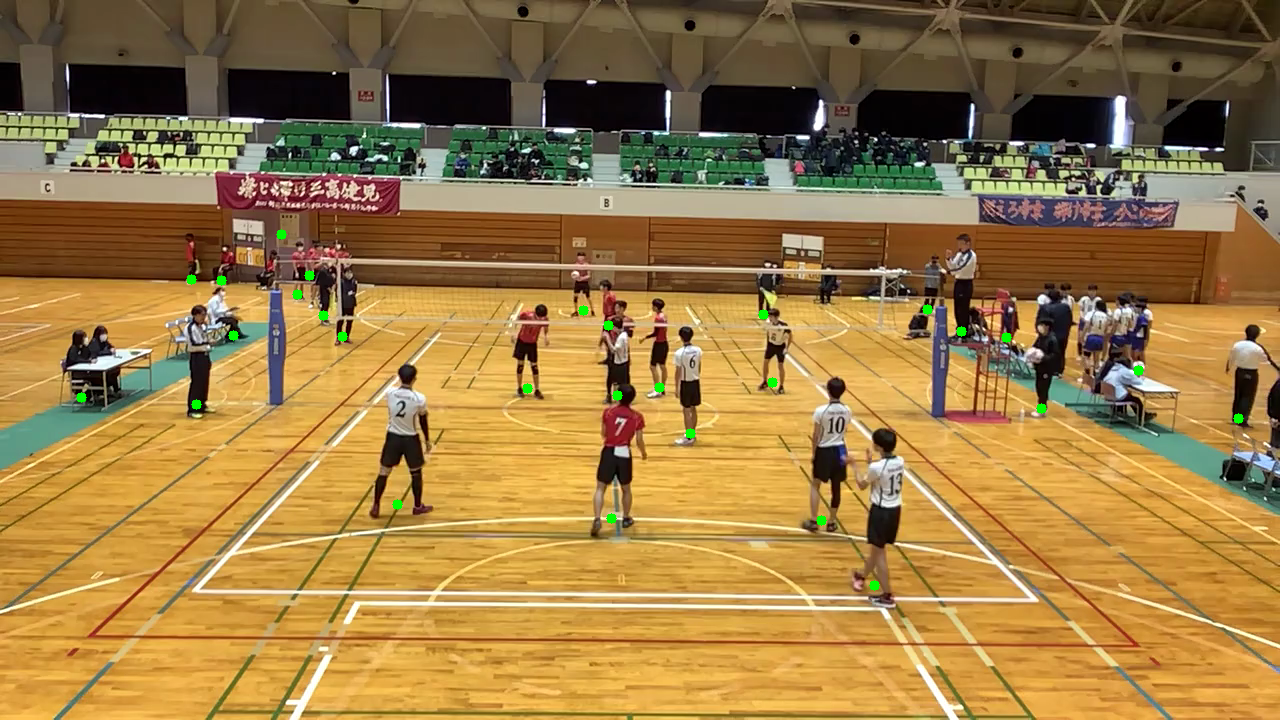
\includegraphics[width=0.9\hsize]{frame.png}
            \caption{試合の画像}
            \label{fig:frame}
        \end{figure}
        \begin{figure}[h]
            \centering
            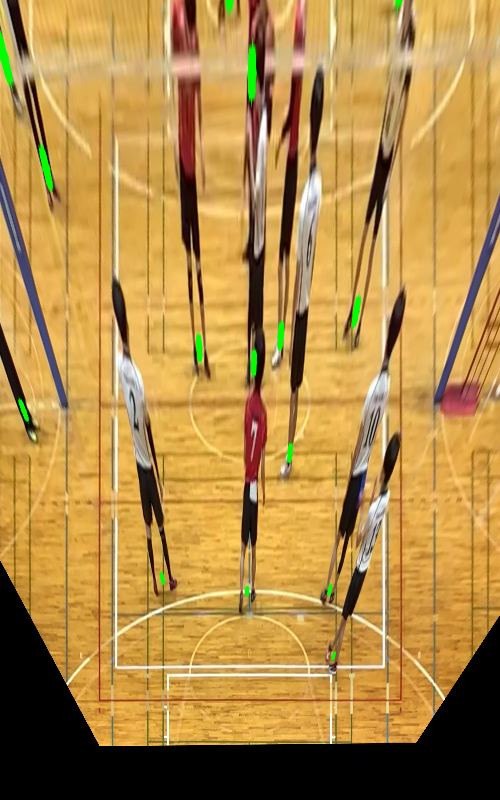
\includegraphics[width=0.5\hsize]{warped.png}
            \caption{射影変換した画像}
            \label{fig:warped}
        \end{figure}

        これらの画像では、AlphaPoseを用いて検出した選手の両足の中間地点
        を選手の床上の位置として緑色にマークしてある。
        画像から分かるように、射影変換を施すと、
        マークが平面上の位置に移動していることがわかる。
        このことを用いて、画像内での選手の位置に同様の射影変換を施して選手の実際の位置とした。

	\subsection{推定位置の精度評価}
        \ref{sec:pos}節で述べたアルゴリズムの推定精度を評価する。
        精度を評価するにあたって、選手の推定位置と、同時刻の実際の位置が必要であるが、
        選手の位置を正確に追跡することは困難であるので、コートのラインが交差している点など、
        いくつかの基準点を設定し、そこに選手がいた瞬間に注目し、精度を評価した。
        %用いた基準点を図\ref{fig:points}に示す。
        用いた基準点は以下のとおりである。

        \begin{enumerate}
            \item 左サイドラインとアタックラインの交点
            \item 左サイドラインとエンドラインの交点
            \item 右サイドラインとアタックラインの交点
            \item 右サイドラインとエンドラインの交点
            \item アタックライン中心
            \item エンドライン中心
        \end{enumerate}
        
        また、カメラの位置による精度の変化を調べるために、
        図\ref{fig:frame}のようにコートの正面からの他に、
        コートの中心と左右それぞれの手前のコートの角を結んだ直線上の
        計3箇所から撮影した映像を用いた。

        %\begin{figure}[h]
        %    \centering
        %    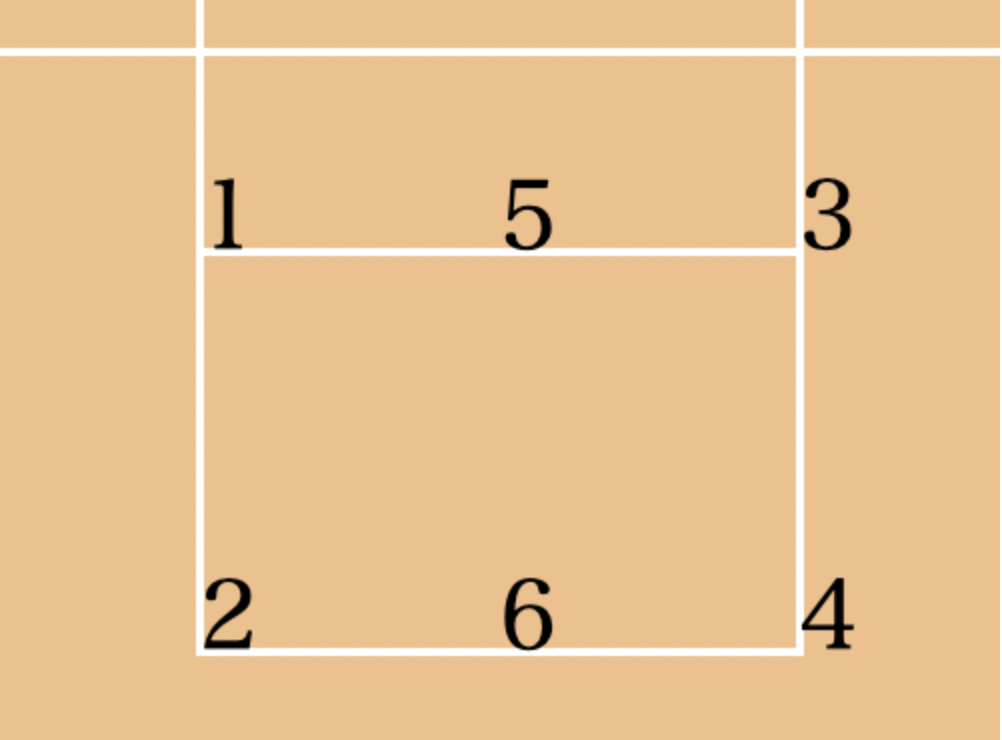
\includegraphics[width=0.9\hsize]{points.png}
        %    \caption{精度測定に用いた基準点}
        %    \label{fig:points}
        %\end{figure}

\section{研究結果}
    図\ref{fig:estimation}に図\ref{fig:frame}に映っている選手らの位置を推定した結果を示す。
    審判含め、コート周辺の人物の位置が
    人間の目で見て違和感のない程度に推定できていることがわかる。

    \begin{figure}[h]
        \centering
        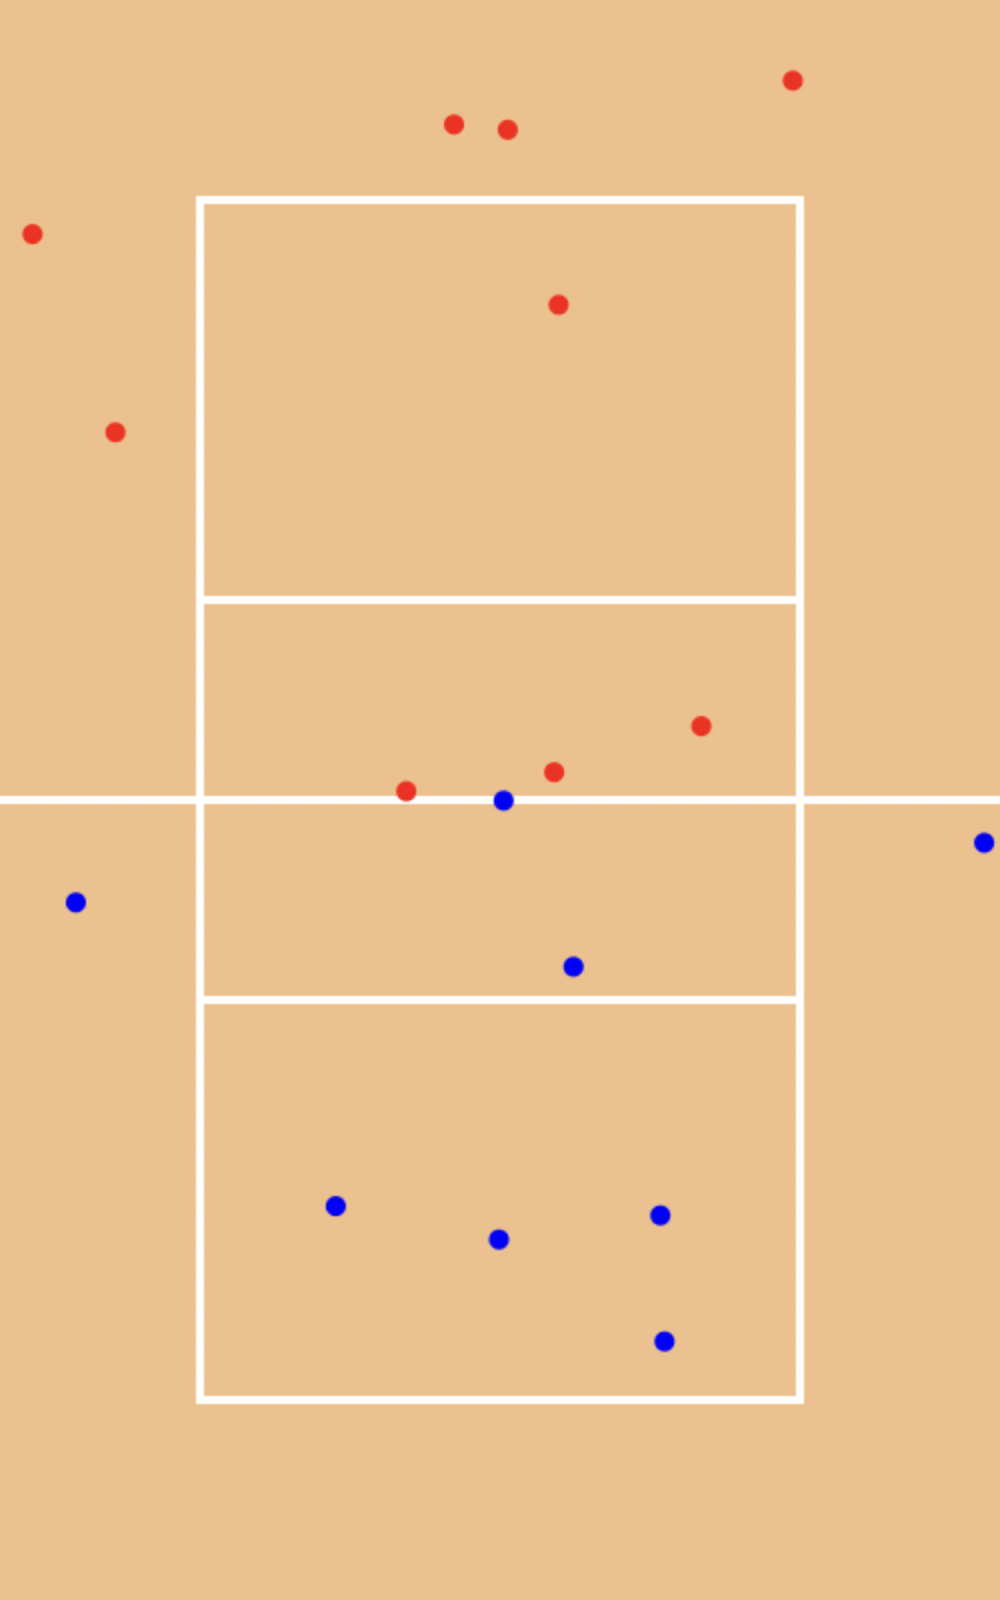
\includegraphics[width=0.4\hsize]{estimated.png}
        \caption{選手の位置推定結果}
        \label{fig:estimation}
    \end{figure}

    表\ref{tab:accuracy_front}、
    \ref{tab:accuracy_left}、\ref{tab:accuracy_right}
    に精度の評価結果を示す。
    表中の番号は基準点の番号で、先述のものと対応している。

    今回撮影に用いたカメラはApple社のiPad Pro内蔵のもので、
    映像の解像度はFHDである。
    また、カメラとコート中心の距離は20mである。

    \begin{table}[h]
        \caption{位置推定の精度[m] 正面から撮影}
        \label{tab:accuracy_front}
        \centering
        \small
        \begin{tabular}{c|cccccc}
            コート & 1 & 2 & 3 & 4 & 5 & 6 \\ \hline \hline
            手前 & 0.15 & 0.18 & 0.14 & 0.12 & 0.13 & 0.10 \\
            奥 & 0.27 & 0.32 & 0.24 & 0.29 & 0.19 & 0.28
        \end{tabular}
    \end{table}
    \begin{table}[h]
        \caption{位置推定の精度[m] 左斜めから撮影}
        \label{tab:accuracy_left}
        \centering
        \small
        \begin{tabular}{c|cccccc}
            コート & 1 & 2 & 3 & 4 & 5 & 6 \\ \hline \hline
            手前 & 0.13 & 0.12 & 0.16 & 0.14 & 0.15 & 0.13 \\
            奥 & 0.18 & 0.20 & 0.25 & 0.32 & 0.23 & 0.28
        \end{tabular}
    \end{table}
    \begin{table}[h]
        \caption{位置推定の精度[m] 右斜めから撮影}
        \label{tab:accuracy_right}
        \centering
        \small
        \begin{tabular}{c|cccccc}
            コート & 1 & 2 & 3 & 4 & 5 & 6 \\ \hline \hline
            手前 & 0.17 & 0.15 & 0.13 & 0.13 & 0.14 & 0.14 \\
            奥 & 0.25 & 0.30 & 0.16 & 0.22 & 0.22 & 0.27
        \end{tabular}
    \end{table}

    表より、カメラとの距離が遠い基準点の精度ほど低下していることがわかる。
    次に、図\ref{fig:distribution}に正面から撮影した際の基準点1に注目した
    各サンプルの推定点の分布を示す。推定点は、縦長の楕円状に分布している。
    これは画像内でコートが縦向きに引き伸ばされており、
    射影変換をした際に横方向より縦方向の誤差が大きく現れたためであると考えられる。
    他の基準点でも同様の分布を示した。

    \begin{figure}[h]
        \centering
        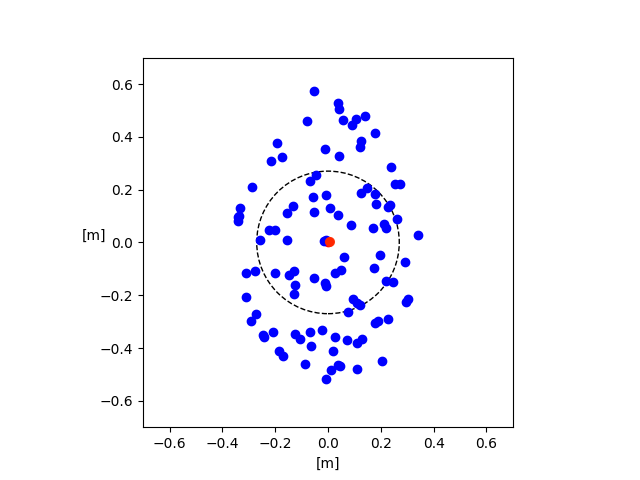
\includegraphics[width=0.9\hsize]{conf.png}
        \caption{推定点の分布}
        \label{fig:distribution}
    \end{figure}

    中心の赤い点が正確な位置で、青い点で示されているのが
    各サンプルの推定点である。
    また、点線は半径が分布の平均値の円である。

\section{まとめ・今後の課題}
    本研究では情報端末の内蔵カメラの映像のみを用いてバレーボールのコート内
    の選手の位置を推定することに成功した。
    これを用いてデータバレーのようなシステムを構築することで人為的ミスの余地のないデータ解析を
    行うことができる。

    また、選手の位置だけでなく姿勢情報も利用することで、試合の3次元再現に発展させられると予想する。

\begin{thebibliography}{99}
    \small {
        \bibitem{Fang}{
			Fang Hao-Shu et al.
			``RMPE: Regional Multi-person Pose Estimation'',
			2017, ICCV
		}
        \bibitem{Redmon}{
			J. Redmon et al.
			``You Only Look Once: Unified, Real-Time Object Detection'',
			2016, CVPR, pp. 779-788.
		}
    }
\end{thebibliography}
\end{document}
